\documentclass[onlymath]{beamer}
% \documentclass[onlymath,handout]{beamer}

% Macros used by all lectures, but not necessarily by excercises

%%% General setup and dependencies:

% \usetheme[ddcfooter,nosectionnum]{tud}
\usetheme[nosectionnum,pagenum,noheader]{tud}
% \usetheme[nosectionnum,pagenum]{tud}

% Increase body font size to a sane level:
\let\origframetitle\frametitle
% \renewcommand{\frametitle}[1]{\origframetitle{#1}\normalsize}
\renewcommand{\frametitle}[1]{\origframetitle{#1}\fontsize{10pt}{13.2}\selectfont}
\setbeamerfont{itemize/enumerate subbody}{size=\small} % tud defaults to scriptsize!
\setbeamerfont{itemize/enumerate subsubbody}{size=\small}
% \setbeamerfont{normal text}{size=\small}
% \setbeamerfont{itemize body}{size=\small}

\renewcommand{\emph}[1]{\textbf{#1}}

\def\arraystretch{1.3}% Make tables even less cramped vertically

\usepackage[ngerman]{babel}
\usepackage[utf8]{inputenc}
\usepackage[T1]{fontenc}

%\usepackage{graphicx}
\usepackage[export]{adjustbox} % loads graphicx
\usepackage{import}
\usepackage{stmaryrd}
\usepackage[normalem]{ulem} % sout command
% \usepackage{times}
\usepackage{txfonts}
\usepackage{array}

% \usepackage[perpage]{footmisc} % reset footnote counter on each page -- fails with beamer (footnotes gone)
\usepackage{perpage}  % reset footnote counter on each page
\MakePerPage{footnote}

\usepackage{tikz}
\usetikzlibrary{arrows,positioning,decorations.pathreplacing}
% Inspired by http://www.texample.net/tikz/examples/hand-drawn-lines/
\usetikzlibrary{decorations.pathmorphing}
\pgfdeclaredecoration{penciline}{initial}{
    \state{initial}[width=+\pgfdecoratedinputsegmentremainingdistance,
    auto corner on length=1mm,]{
        \pgfpathcurveto%
        {% From
            \pgfqpoint{\pgfdecoratedinputsegmentremainingdistance}
                      {\pgfdecorationsegmentamplitude}
        }
        {%  Control 1
        \pgfmathrand
        \pgfpointadd{\pgfqpoint{\pgfdecoratedinputsegmentremainingdistance}{0pt}}
                    {\pgfqpoint{-\pgfdecorationsegmentaspect
                     \pgfdecoratedinputsegmentremainingdistance}%
                               {\pgfmathresult\pgfdecorationsegmentamplitude}
                    }
        }
        {%TO
        \pgfpointadd{\pgfpointdecoratedinputsegmentlast}{\pgfpoint{1pt}{1pt}}
        }
    }
    \state{final}{}
}
\tikzset{handdrawn/.style={decorate,decoration=penciline}}
\tikzset{every shadow/.style={fill=none,shadow xshift=0pt,shadow yshift=0pt}}
% \tikzset{module/.append style={top color=\col,bottom color=\col}}

% Use to make Tikz attributes with Beamer overlays
% http://tex.stackexchange.com/a/6155
\tikzset{onslide/.code args={<#1>#2}{%
  \only<#1| handout:0>{\pgfkeysalso{#2}}
}}
\tikzset{onslideprint/.code args={<#1>#2}{%
  \only<#1>{\pgfkeysalso{#2}}
}}

%%% Title -- always set this first

\newcommand{\defineTitle}[3]{
	\newcommand{\lectureindex}{#1}
	\title{Theoretische Informatik und Logik}
	\subtitle{\href{\lectureurl}{#1. Vorlesung: #2}}
	\author{\href{https://iccl.inf.tu-dresden.de/web/Markus_Kr\%C3\%B6tzsch}{Markus Kr\"{o}tzsch}\\[1ex]Lehrstuhl Wissensbasierte Systeme}
	\date{#3}
	\datecity{TU Dresden}
% 	\institute{CC-By 3.0, sofern keine anderslautenden Bildrechte angegeben sind}
}

%%% Table of contents:

\RequirePackage{ifthen}

\newcommand{\highlight}[2]{%
	\ifthenelse{\equal{#1}{\lectureindex}}{\alert{#2}}{#2}%
}

\def\myspace{-0.7ex}
\newcommand{\printtoc}{
\begin{tabular}{r@{$\quad$}l}
\highlight{1}{1.} & \highlight{1}{Willkommen/Einleitung formale Sprachen}\\[\myspace]
\highlight{2}{2.} & \highlight{2}{Grammatiken und die Chomsky-Hierarchie}\\[\myspace]
\highlight{3}{3.} & \highlight{3}{Endliche Automaten}\\[\myspace]
\highlight{4}{4.} & \highlight{4}{Complexity of FO query answering}\\[\myspace]
\highlight{5}{5.} & \highlight{5}{Conjunctive queries}\\[\myspace]
\highlight{6}{6.} & \highlight{6}{Tree-like conjunctive queries}\\[\myspace]
\highlight{7}{7.} & \highlight{7}{Query optimisation}\\[\myspace]
\highlight{8}{8.} & \highlight{8}{Conjunctive Query Optimisation / First-Order~Expressiveness}\\[\myspace]
\highlight{9}{9.} & \highlight{9}{First-Order~Expressiveness / Introduction to Datalog}\\[\myspace]
\highlight{10}{10.} & \highlight{10}{Expressive Power and Complexity of Datalog}\\[\myspace]
\highlight{11}{11.} & \highlight{11}{Optimisation and Evaluation of Datalog}\\[\myspace]
\highlight{12}{12.} & \highlight{12}{Evaluation of Datalog (2)}\\[\myspace]
\highlight{13}{13.} & \highlight{13}{Graph Databases and Path Queries}\\[\myspace]
\highlight{14}{14.} & \highlight{14}{Outlook: database theory in practice}
\end{tabular}
}

\newcommand{\overviewslide}{%
\begin{frame}\frametitle{Overview}
\printtoc
\medskip

Siehe \href{\lectureurl}{course homepage [$\Rightarrow$ link]} for more information and materials
\end{frame}
}

%%% Colours:
\usepackage{xcolor,colortbl}
\definecolor{redhighlights}{HTML}{FFAA66}
\definecolor{lightblue}{HTML}{55AAFF}
\definecolor{lightred}{HTML}{FF5522}
\definecolor{lightpurple}{HTML}{DD77BB}
\definecolor{lightgreen}{HTML}{55FF55}
\definecolor{darkred}{HTML}{CC4411}
\definecolor{darkblue}{HTML}{176FC0}%{1133AA}
\definecolor{nightblue}{HTML}{2010A0}%{1133AA}
\definecolor{alert}{HTML}{176FC0}
\definecolor{darkgreen}{HTML}{36AB14}
\definecolor{strongyellow}{HTML}{FFE219}
\definecolor{devilscss}{HTML}{666666}

\newcommand{\redalert}[1]{\textcolor{darkred}{#1}}

%%% Slide layout commands:

\newcommand{\sectionSlide}[1]{
\frame{\begin{center}
\LARGE
#1
\end{center}}
}
\newcommand{\sectionSlideNoHandout}[1]{
\frame<handout:0>{\begin{center}
\LARGE
#1
\end{center}}
}

\newcommand{\mydualbox}[3]{%
 \begin{minipage}[t]{#1}
 \begin{beamerboxesrounded}[upper=block title,lower=block body,shadow=true]%
    {\centering\usebeamerfont*{block title}#2}%
    \raggedright%
    \usebeamerfont{block body}
%     \small
    #3%
  \end{beamerboxesrounded}
  \end{minipage}
}
%
\newcommand{\myheaderbox}[2]{%
 \begin{minipage}[t]{#1}
 \begin{beamerboxesrounded}[upper=block title,lower=block title,shadow=true]%
    {\centering\usebeamerfont*{block title}\rule{0pt}{2.6ex} #2}%
  \end{beamerboxesrounded}
  \end{minipage}
}

\newcommand{\mycontentbox}[2]{%
 \begin{minipage}[t]{#1}%
 \begin{beamerboxesrounded}[upper=block body,lower=block body,shadow=true]%
    {\centering\usebeamerfont*{block body}\rule{0pt}{2.6ex}#2}%
  \end{beamerboxesrounded}
  \end{minipage}
}

\newcommand{\mylcontentbox}[2]{%
 \begin{minipage}[t]{#1}%
 \begin{beamerboxesrounded}[upper=block body,lower=block body,shadow=true]%
    {\flushleft\usebeamerfont*{block body}\rule{0pt}{2.6ex}#2}%
  \end{beamerboxesrounded}
  \end{minipage}
}

% label=180:{\rotatebox{90}{{\footnotesize\textcolor{darkgreen}{Beispiel}}}}
% \hspace{-8mm}\ghost{\raisebox{-7mm}{\rotatebox{90}{{\footnotesize\textcolor{darkgreen}{Beispiel}}}}}\hspace{8mm}
\newcommand{\examplebox}[1]{%
	\begin{tikzpicture}[decoration=penciline, decorate]
		\pgfmathsetseed{1235}
		\node (n1) [decorate,draw=darkgreen, fill=darkgreen!10,thick,align=left,text width=\linewidth, inner ysep=2mm, inner xsep=2mm] at (0,0) {#1};
% 		\node (n2) [align=left,text width=\linewidth,inner sep=0mm] at (n1.92) {{\footnotesize\raisebox{3mm}{\textcolor{darkgreen}{Beispiel}}}};
% 		\node (n2) [decorate,draw=darkgreen, fill=darkgreen!10,thick, align=left,text width=\linewidth,inner sep=2mm] at (n1.90) {{\footnotesize\raisebox{0mm}{\textcolor{darkgreen}{Beispiel}}}};
	\end{tikzpicture}%
}%

\newcommand{\codebox}[1]{%
	\begin{tikzpicture}[decoration=penciline, decorate]
		\pgfmathsetseed{1236}
		\node (n1) [decorate,draw=strongyellow, fill=strongyellow!10,thick,align=left,text width=\linewidth, inner ysep=2mm, inner xsep=2mm] at (0,0) {#1};
	\end{tikzpicture}%
}%

\newcommand{\defbox}[1]{%
	\begin{tikzpicture}[decoration=penciline, decorate]
		\pgfmathsetseed{1237}
		\node (n1) [decorate,draw=darkred, fill=darkred!10,thick,align=left,text width=\linewidth, inner ysep=2mm, inner xsep=2mm] at (0,0) {#1};
	\end{tikzpicture}%
}%

\newcommand{\theobox}[1]{%
	\begin{tikzpicture}[decoration=penciline, decorate]
		\pgfmathsetseed{1240}
		\node (n1) [decorate,draw=darkblue, fill=darkblue!10,thick,align=left,text width=\linewidth, inner ysep=2mm, inner xsep=2mm] at (0,0) {#1};
	\end{tikzpicture}%
}%

\newcommand{\anybox}[2]{%
	\begin{tikzpicture}[decoration=penciline, decorate]
		\pgfmathsetseed{1240}
		\node (n1) [decorate,draw=#1, fill=#1!10,thick,align=left,text width=\linewidth, inner ysep=2mm, inner xsep=2mm] at (0,0) {#2};
	\end{tikzpicture}%
}%


\newsavebox{\mybox}%
\newcommand{\doodlebox}[2]{%
\sbox{\mybox}{#2}%
	\begin{tikzpicture}[decoration=penciline, decorate]
		\pgfmathsetseed{1238}
		\node (n1) [decorate,draw=#1, fill=#1!10,thick,align=left,inner sep=1mm] at (0,0) {\usebox{\mybox}};
	\end{tikzpicture}%
}%


\defineTitle{21}{Endliche Modelle/ Gödels~1.~Unvollständigkeitssatz}{5. Juli 2017}

\begin{document}

\maketitle




\frame{\label{frame_goedel}\begin{center}
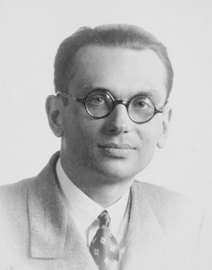
\includegraphics[height=5cm]{images/Goedel.jpg}

\LARGE
Kurt Gödel
\end{center}}


\begin{frame}\frametitle{Der 1. Gödelsche Unvollständigkeitssatz}

Was Gödel in 1931 zeigte war grob gesagt folgendes:\medskip

\theobox{Satz: Jedes konsistente formale System, in dem eine gewisse Menge elementarer Arithmetik
dargestellt werden kann, ist unvollständig in Bezug auf die Beweisbarkeit von Sätzen der
elementaren Arithmetik: Es gibt solche Sätze, die weder bewiesen noch widerlegt werden können.
}\bigskip

\emph{Um das zu verstehen müssen wir einiges klären:}
\begin{itemize}
\item Was ist ein \alert{formales System}?
\item Was ist \alert{konsistent}?
\item Was ist \alert{"`eine gewisse Menge elementarer Arithmetik"'}?
\item Was genau bedeutet \alert{unvollständig} hier?
\end{itemize}

\end{frame}

\begin{frame}\frametitle{Formale Systeme}

Ein \redalert{formales System} ist ganz allgemein ein Beweissystem, bestehend aus:
\begin{itemize}
\item Einer Sprache, in der Aussagen formuliert werden können
\item Einer Menge von Axiomen, d.h. als wahr vorgegebener Aussagen
\item Einem effektiven Verfahren mit dem man aus gegebenen Aussagen neue Schlüsse ableiten kann
\end{itemize}
Beweisbare Sätze heißen \redalert{Theoreme} des formalen Systems\\
{\tiny {\emph{Anmerkung:} Auch die Axiome sind Theoreme, wenn auch mit sehr kurzen Beweisen}}
\medskip\pause

\examplebox{Beispiel: Prädikatenlogik liefert formales Systeme:
\begin{itemize}
\item Sprache: Die Sprache der prädikatenlogischen Sätze
\item Axiome: Eine gegebene Theorie, z.B. die Theorie der kommutativen Monoide
\item Ableitungsverfahren: Resolutionskalkül
\end{itemize}
}



\end{frame}


\begin{frame}\frametitle{Formale Systeme: Wichtige Eigenschaften}

Formale Systeme können viele Formen haben -- zum Beispiel beinhalten sie auch jedes System, in dem mathematische Beweise formal geführt werden können (z.B. ZFC: Mengenlehre nach Zermelo-Fraenkel mit Auswahlaxiom).\bigskip\pause

Die Details sind relativ egal, aber
wir wollen doch ein paar Anforderungen stellen:

\anybox{purple}{Grundeigenschaft Formaler Systeme: Die Menge der Theoreme eines formalen Systems ist rekursiv aufzählbar (semi-entscheidbar).}

\anybox{purple}{Negation: Für jeden Satz $S$ gibt es in der Sprache eines formalen Systems auch einen negierten Satz $\neg S$, so dass gilt:
\begin{itemize}
\item $S$ ist genau dann ein Theorem, wenn $\neg\neg S$ ein Theorem ist.
\item Wenn $S$ und $\neg S$ Theoreme sind, dann sind alle Sätze Theoreme.
\end{itemize}
}

\end{frame}

\begin{frame}\frametitle{Eigenschaften formaler Systeme}


\emph{Syntaktische Eigenschaften:}
\begin{itemize}
\item \redalert{Konsistenz:} Ein formales System ist konsistent, wenn es keinen Satz $S$ gibt,
so dass $S$ und $\neg S$ beweisbar sind.
\item \redalert{Vollständigkeit:} Ein formales System ist (negations-)vollständig, wenn für jeden Satz $S$ entweder $S$ oder $\neg S$ beweisbar sind.
\end{itemize}
% Bisher haben wir keinerlei Semantik definiert oder verwendet. Diese Eigenschaften beziehen sich nur auf die Syntax der mechanisch ableitbaren Formeln.
\medskip\pause

Wenn man z.B. in Prädikatenlogik arbeitet, dann kann man Mengen von Sätzen eine Semantik (Modelltheorie) geben und weitere Eigenschaften fordern:\medskip

\emph{Semantische Eigenschaften:}
\begin{itemize}
\item \redalert{Korrektheit:} Ein formales System ist korrekt, wenn jeder beweisbare Satz auch semantisch wahr (tautologisch) ist.
\item \redalert{Vollständigkeit:} Ein formales System ist (semantisch) vollständig, wenn jeder semantisch wahre Satz beweisbar ist.
\end{itemize}

\end{frame}

\begin{frame}\frametitle{Verwechslungsgefahr}

\anybox{purple}{
\emph{Achtung!} Es gibt zwei Arten von Vollständigkeit:
\begin{itemize}
\item Negationsvollständigkeit: die syntaktische Eigenschaft, dass jeder Satz bewiesen oder widerlegt werden kann
\item Semantische Vollständigkeit: die semantische Eigenschaft, dass jede Tautologie bewiesen werden kann
\end{itemize}

Gödels Vollständigkeitssatz bezieht sich auf die zweite Art von Vollständigkeit,
Gödels Unvollständigkeitssätze auf die erste!}

\end{frame}


\begin{frame}\frametitle{Beispiele}

\examplebox{Beispiel: Angenommen ein Satz $F$ kann in einem formalen System
$\mathcal{S}$ bewiesen und wir wissen, dass $\mathcal{S}$ konsistent ist.
Folgt daraus, dass $F$ semantisch wahr ist?
}\medskip\pause

\examplebox{Beispiel: Aus der Logik bekannte Zusammenhänge gelten auch hier:
\begin{itemize}
\item Ein Satz $F$ ist genau dann in $\mathcal{S}$ beweisbar wenn $\mathcal{S}$ bei Hinzunahme des Axioms $\neg F$ inkonsistent wird.
\item Weder $F$ noch $\neg F$ sind in $\mathcal{S}$ beweisbar gdw. $\mathcal{S}$ sowohl bei Hinzunahme von $F$ als auch bei Hinzunahme von $\neg F$ konsistent ist
\end{itemize}
}


\end{frame}

\begin{frame}\frametitle{Eine gewisse Menge Arithmetik}

\theobox{Satz: Jedes konsistente formale System, in dem eine gewisse Menge elementarer Arithmetik
dargestellt werden kann, ist unvollständig in Bezug auf die Beweisbarkeit von Sätzen der
elementaren Arithmetik: Es gibt solche Sätze, die weder bewiesen noch widerlegt werden können.
}

Was ist mit "`eine gewisse Menge elementarer Arithmetik"' gemeint?\pause
\begin{itemize}
\item Das System sollte Sätze über Beziehungen von konkreten natürlichen Zahlen ausdrücken können
\item Dabei sollten die elementaren Operationen $+$, $-$ und $\times$ sowie die Relation $=$ unterstützt werden
\item Das System sollte bezüglich der gängigen Semantik dieser arithmetischen Ausdrucksmittel korrekt sein
\end{itemize}
Oft kommt man mit noch weniger aus, aber diese Eigenschaften reichen in der Regel

\end{frame}

\begin{frame}\frametitle{Arithmetik in Prädikatenlogik}

Man kann die benötigte Menge von Arithmetik durch eine prädikatenlogische Theorie axiomatisieren:
\begin{itemize}
\item Konstante $\Sterm{0}$
\item Funktionssymbole $s$ (unär, "`Nachfolger"'), $+$ und $\times$ (binär, infix)
\item Prädikatssymbol $\approx$ (binär, infix)
\end{itemize}

Darstellung natürlicher Zahlen als Nachfolger von 0:\\[0.5ex]
\narrowcentering{$\Sterm{0}\hat{=}0$, $s(\Sterm{0})\hat{=}1$, $s(s(\Sterm{0}))\hat{=}2$, \ldots}\bigskip

Sätze zur Axiomaitiserung der Grundrechenarten:
\begin{itemize}
\item $\forall x.\neg(s(x)\approx \Sterm{0})$
\item $\forall x.(x+\Sterm{0}\approx x)$ 
\item $\forall x,y.(x+s(y)\approx s(x+y))$
\item $\forall x.(x\times \Sterm{0}\approx \Sterm{0})$ 
\item $\forall x,y.(x\times s(y)\approx (x\times y)+x$
\item \ldots {\tiny (mit obigem kann man schon einiges ausrechnen, aber es gibt noch mehr zu sagen, z.B. eine komplette Gleichheitstheorie)

}
\end{itemize}

\end{frame}

\sectionSlide{Gödels Beweis des 1. Satzes}

\begin{frame}\frametitle{Idee}

Wie kann man zeigen, dass irgendein Satz weder beweisbar noch widerlegbar ist?
\bigskip\pause

\emph{Ein einfaches Szenario:}
\begin{itemize}
\item \alert{Annahme:} Sie glauben nur Dinge, die wirklich wahr sind, und was Sie glauben ist konsistent.\pause
\item \alert{Behauptung:} Es gibt wahre Sätze, die sie nicht glauben.\pause
\item \alert{Beweis:}\pause "`Ich mache jetzt eine wahre Behauptung, die Sie mir nicht glauben"'\pause{} ist eine Behauptung, die sie nicht glauben können:
\begin{itemize}
\item Wenn Sie sie glauben, dann muss sie wahr sein, d.h. Sie glauben sie nicht -- das wäre inkonsistent
\item Also glauben Sie sie nicht. Dann ist die Behauptung wahr.\qed
\end{itemize}
\end{itemize}

Behauptungen dieser Form nennt man \redalert{Gödelsätze}

\end{frame}

\begin{frame}\frametitle{Gödelsätze formal machen}

Natürliche Sprache eignet sich nicht für stichhaltige Argumente, da sie keine klar definierte mathematische Interpretation hat (z.B. kann ich sagen "`Dieser Satz ist eine Lüge"')
\bigskip\pause

Gödels Beweis (vereinfacht) für formale Systeme:
\begin{itemize}
\item \alert{Annahme:} Das gegebene System ist korrekt und konsistent.
\item \alert{Behauptung:} Es gibt wahre Sätze, die nicht beweisbar sind.
\item \alert{Beweis:} Gödel definiert eine mathematische Formel $F$, welche ausdrückt:\\[1ex]
\narrowcentering{\alert{"`$F$ ist wahr genau dann wenn $F$ nicht beweisbar ist."'}}\smallskip

\begin{itemize}
\item Wenn $F$ beweisbar wäre, dann ist es wahr und also nicht beweisbar -- Widerspruch
\item Also ist $F$ nicht beweisbar, und damit wahr\qed
\end{itemize}
\end{itemize}

\end{frame}

\begin{frame}\frametitle{Gödels Zahlen}

\narrowcentering{\alert{"`$F$ ist wahr genau dann wenn $F$ nicht beweisbar ist."'}}\smallskip

Die Herausforderung ist, solche Gödensätze zu definieren:
Offenbar kann man $F$ nicht als Teilausdruck in $F$ verwenden!
\bigskip\pause

Gödel definiert daher nummerische Bezeichner für Formeln -- sogenannte Gödelzahlen -- und kodiert seine Sätze anders:
\begin{center}\alert{"`$F$ ist wahr genau dann wenn $m$ in der Menge der Gödelzahlen nicht beweisbarer Sätze vorkommt."'} \end{center}
wobei $m$ die Gödelzahl für $F$ ist.\medskip

Man muss dafür eine Menge technischer Ergebnisse zeigen, z.B.
\begin{itemize}
\item Ein solcher Satz $F$, welcher seine eigene Gödelzahl verwendet, existiert überhaupt
\item Die Menge der Gödelzahlen nicht beweisbarer Sätze ist arithmetisch darstellbar
\end{itemize}

\end{frame}


\begin{frame}\frametitle{Quotes und Quines}

Eine verwandte Form von Selbstbezüglichkeit ist auch in der Informatik bekannt:\medskip

\defbox{
Ein \redalert{Quine} ist ein Programm, das bei einer leeren Eingabe seinen eigenen Quellcode ausgibt.
}

Auch hier denkt man vielleicht zuerst, dass dies nicht möglich wäre, weil das Programm dazu seinen eigenen Code enthalten müsste -- eine unendliche Rekursion \ldots\medskip
\pause

Es ist aber gar nicht so schwer:
\bigskip
\examplebox{Beispiel: Gib den folgenden Satz zweimal aus, beim zweiten mal in Anführungszeichen: $\squote$Gib den folgenden Satz zweimal aus, beim zweiten mal in Anführungszeichen: $\squote$ }

\end{frame}

\sectionSlide{Gödels 1. Satz berechnungstheoretisch zeigen}

\begin{frame}\frametitle{Unentscheidbarkeit und Unvollständigkeit}

\emph{Wir wissen:}\medskip

Die Theoreme formaler Systeme sind rekursiv aufzählbar, d.h. semi-entscheidbar
\begin{itemize}
\item Speziell gilt das auch für die Theoreme, die sich auf arithmetische Aussagen beziehen
\end{itemize}\medskip

Es gibt Mengen (Sprachen), die nicht semi-entscheidbar sind
\begin{itemize}
\item Zum Beispiel das Nicht-Halteproblem von Turingmaschinen
\end{itemize}
\bigskip\pause

\alert{
$\leadsto$ Falls man Instanzen des Wortproblems einer nicht-semientscheidbaren Sprache auf die Wahrheit arithmetischer Sätze reduzieren könnte, dann würde daraus schon Unvollständigkeit folgen}

\end{frame}

\begin{frame}\frametitle{Zahlen vs. Sprachen}

Berechnungstheorie handelt von Sprachen, d.h. Mengen von Wörtern
\bigskip

Es ist leicht möglich, jedem Wort eine natürliche Zahl zuzuordnen -- man spricht von einer \redalert{Gödelzahl} für das Wort\\[0.5ex]
{\tiny(dies ist möglich, da die Menge aller Wörter abzählbar ist, siehe Formale Systeme WS 2016/2017; natürlich gibt es viele mögliche Zuordnungen).

}
\bigskip\pause

Wir folgern:
\begin{itemize}
\item Es gibt eine Eins-zu-eins-Beziehung zwischen formalen Sprachen (über einem gegebenen Alphabet) und Mengen natürlicher Zahlen
\item Wir können also von der Entscheidbarkeit/Unentscheidbarkeit einer Menge natürlicher Zahlen sprechen
\item Es gibt unentscheidbare Mengen natürlicher Zahlen, z.B. die Menge der Zahlen, welche ein Wort enummieren, das eine Turingmaschine kodiert, welche auf der leeren Eingabe hält
\end{itemize}

\end{frame}

\begin{frame}\frametitle{Eine erste Beweisidee}

Mögliche Strategie zum Beweis von Gödels 1. Satz:
\begin{itemize}
\item Definiere eine Gödel-Nummerierung für alle Wörter die eine Turingmaschine kodieren
\item Finde arithmetische Ausdrücke auf diesen Zahlen, mit denen man konkrete syntaktische Eigenschaften der kodierten TM testen kann
\item Finde arithmetische Formeln, die ausdrücken, dass die kodierte TM auf dem leeren Wort hält
\end{itemize}\pause
\alert{$\leadsto$ Programmiere eine universelle TM in Arithmetik}\bigskip

(Machbar, aber aufwändig!)

\end{frame}

\begin{frame}\frametitle{Ein schweres arithmetisches Problem}

Die Aufgabe wird viel einfacher, wenn man mit ein unentscheidbares Problem verwendet, welches sich schon auf arithmetische Aussagen bezieht.

\defbox{Eine \redalert{Diophantische Gleichung} ist ein arithmetischer Ausdruck der Form $D[x_1,\ldots,x_n]= 0$, wobei $D[x_1,\ldots,x_n]$ ein Funktionsterm über den Symbolen
$x_1,\ldots,x_n,\Sterm{0},s,+,-,\times$ ist. Eine \redalert{Lösung} der Gleichung ist eine Liste von natürlichen Zahlen $z_1,\ldots,z_n$, für welche die Gleichung stimmt.}\pause

\examplebox{Beispiele für diophantische Gleichungen:
\begin{itemize}
\item $y=3x+5$, d.h. $3\times x-y+5= 0$ (unendlich viele Lösungen)
\item $x^2+y^2= -1$, d.h. $x\times x+y\times y+1 = 0$ (keine Lösung)
\item $x^2+y^2=z^2$ (unendlich viele Lösungen)
\item $x^4+y^4=z^4$ (genau eine Lösung, Fermatsche Vermutung)
\item $x^2=2y^4-1$ (genau zwei Lösungen: 1 \& 1 und 13 \& 239)
\end{itemize}
}

\end{frame}

\begin{frame}\frametitle{Hilberts Zehntes und MRDP}

\anybox{purple}{Hilberts 10. Problem: Man finde ein Verfahren um zu ermitteln, ob eine gegebene diophantische Gleichung lösbar ist.}\pause

Wir wissen heute, dass dies unentscheidbar ist:
\begin{itemize}
\item Jede diophantische Gleichung $D[x_1,\ldots,x_n,y]= 0$ definiert eine Menge natürlicher Zahlen $\{k\mid D[x_1,\ldots,x_n,k]= 0 \text{ ist lösbar}\}$
\item Eine so definierte Menge heißt \redalert{diophantische Menge}
\item Alle diophantischen Mengen sind rekursiv aufzählbar: teste systematisch alle möglichen Belegungen von $D[x_1,\ldots,x_n,y]= 0$ und gib bei jeder gefundenen Lösung den Wert von $y$ aus
\end{itemize}\pause

\theobox{Satz (Matiyasevich/Robinson/Davis/Putnam): Jede rekursiv aufzählbare Menge natürlicher Zahlen ist diophantisch.}
{\tiny Intuitiv: diophantische Gleichungen sind Turing-mächtig!}

\end{frame}

\begin{frame}\frametitle{Konsequenzen}

\emph{Wir folgern:}
\begin{itemize}
\item \alert{Hilberts 10. Problem ist wirklich unentscheidbar:}
\begin{itemize}
\item Wäre es entscheidbar, dann könnte man jede diophantische Menge entscheiden (Kontrollfrage: Wie?)
\item Wir wissen aber bereits, dass es rekursiv aufzählbare Mengen natürlicher Zahlen gibt, die nicht entscheidbar sind
\end{itemize}\pause
\item \alert{Nicht-Lösbarkeit diophantischer Gleichungen ist nicht semi-entscheidbar:}
\begin{itemize}
\item Lösbarkeit ist bereits semi-entscheidbar
\item Wenn Nicht-Lösbarkeit auch semi-entscheidbar wäre, dann wäre beides entscheidbar
\end{itemize}
\end{itemize}

\end{frame}

\begin{frame}\frametitle{Beweis von Gödels 1. Unvollständigkeitssatz}

Sei $\mathcal{S}$ ein formales System, welches das folgende erfüllt:
\begin{enumerate}[(1)]
\item $\mathcal{S}$ ist konsistent
\item Jede wahre Aussage der Form $D[z_1,\ldots,z_n]= 0$ für eine beliebige diophantische Gleichungen und \alert{konkrete} Zahlenwerte $z_1,\ldots, z_n$ ist beweisbar {\tiny(einfach durch Ausrechnen des Wertes)}
\item Sätze der Form $\exists x_1,\ldots, x_n.D[x_1,\ldots,x_n]= 0$ sind darstellbar und alle beweisbaren Sätze dieser Form sind korrekt
\end{enumerate}\pause
\emph{Wegen (1) und (2) gilt:} $\mathcal{S}$ beweist nur wahre Sätze der Form $\neg\exists x_1,\ldots, x_n.D[x_1,\ldots,x_n]= 0$\medskip\pause

\emph{Aber:} $\mathcal{S}$ kann nicht alle wahren Sätze dieser Form beweisen:
\begin{itemize}
\item Die Menge aller beweisbaren Sätze dieser Form ist semi-entscheidbar
\item Die Menge aller wahren Sätze dieser Form ist nicht semi-entscheidbar
\end{itemize}\pause
\emph{Mit (3) gilt:} Es gibt Sätze $F$ der Form \ghost{$\exists x_1,\ldots, x_n.D[x_1,\ldots,x_n]= 0$,}\\ so dass weder $F$ noch $\neg F$ bewiesen wird.\qed

\end{frame}



\begin{frame}\frametitle{Zusammenfassung und Ausblick}

Das Auswertungsproblem der Prädikatenlogik ist \PSpace-vollständig\bigskip

Formale Systeme, die elementare Rechnungen auf natürlichen Zahlen ausführen können
sind entweder inkonsistent oder (negations-)unvollständig
\bigskip

Diese Unvollständigkeit hat damit zu tun, dass nicht alle Mengen natürlicher Zahlen Turing-erkennbar sind\bigskip

\anybox{yellow}{
Was erwartet uns als nächstes?
\begin{itemize}
\item 3. Repetitorium
\item Probeklausur
\item Gödels zweiter Unvollständigkeitssatz, Zusammenfassung und Ausblick
\end{itemize}
}

\end{frame}


\begin{frame}[t]\frametitle{Bildrechte}

Folie \ref{frame_goedel}: Fotografie um 1926, gemeinfrei

\end{frame}


\end{document}
